\documentclass{article}

\usepackage[letterpaper, portrait, margin=1.5in]{geometry}

\usepackage{fancyhdr}
\usepackage{ragged2e}
\usepackage{graphicx}
\usepackage{caption}
\usepackage{amsmath}
\usepackage{rotating}
\usepackage{caption}
\usepackage{subcaption}

\usepackage{listings}
\usepackage{color}

\definecolor{dkgreen}{rgb}{0,0.6,0}
\definecolor{gray}{rgb}{0.5,0.5,0.5}
\definecolor{mauve}{rgb}{0.58,0,0.82}

\lstset{frame=tb,
  language=Java,
  aboveskip=3mm,
  belowskip=3mm,
  showstringspaces=false,
  columns=flexible,
  basicstyle={\small\ttfamily},
  numbers=none,
  numberstyle=\tiny\color{gray},
  keywordstyle=\color{blue},
  commentstyle=\color{dkgreen},
  stringstyle=\color{mauve},
  breaklines=true,
  breakatwhitespace=true,
  tabsize=4
}

\setcounter{secnumdepth}{1}

\usepackage{chngcntr}
\counterwithin{figure}{section}

\renewcommand*{\thepage}{C\arabic{page}}

\pagestyle{fancy}
\lhead{ACME Robotics}
\chead{\#8367}
\rhead{\ifcontents Contents \else Week \thesection \fi}

\newif\ifcontents
\contentstrue

\makeatletter
\renewcommand{\@seccntformat}[1]{}
\makeatother
\begin{document}

\begin{figure}[h!]
\centering
\begin{subfigure}{.5\textwidth}
  \centering
  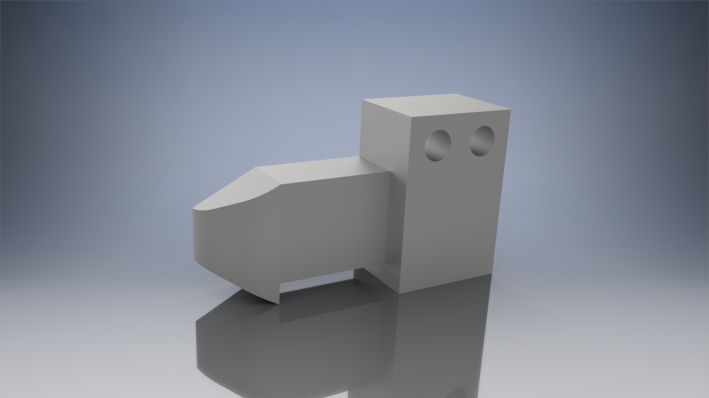
\includegraphics[width=\textwidth,]{27_03-04/images/latchCAD.png}
  \caption{CAD Latch Stress Analysis}
  \label{fig:Latch}
 \end{subfigure}
\begin{subfigure}{.35\textwidth}
  \centering
  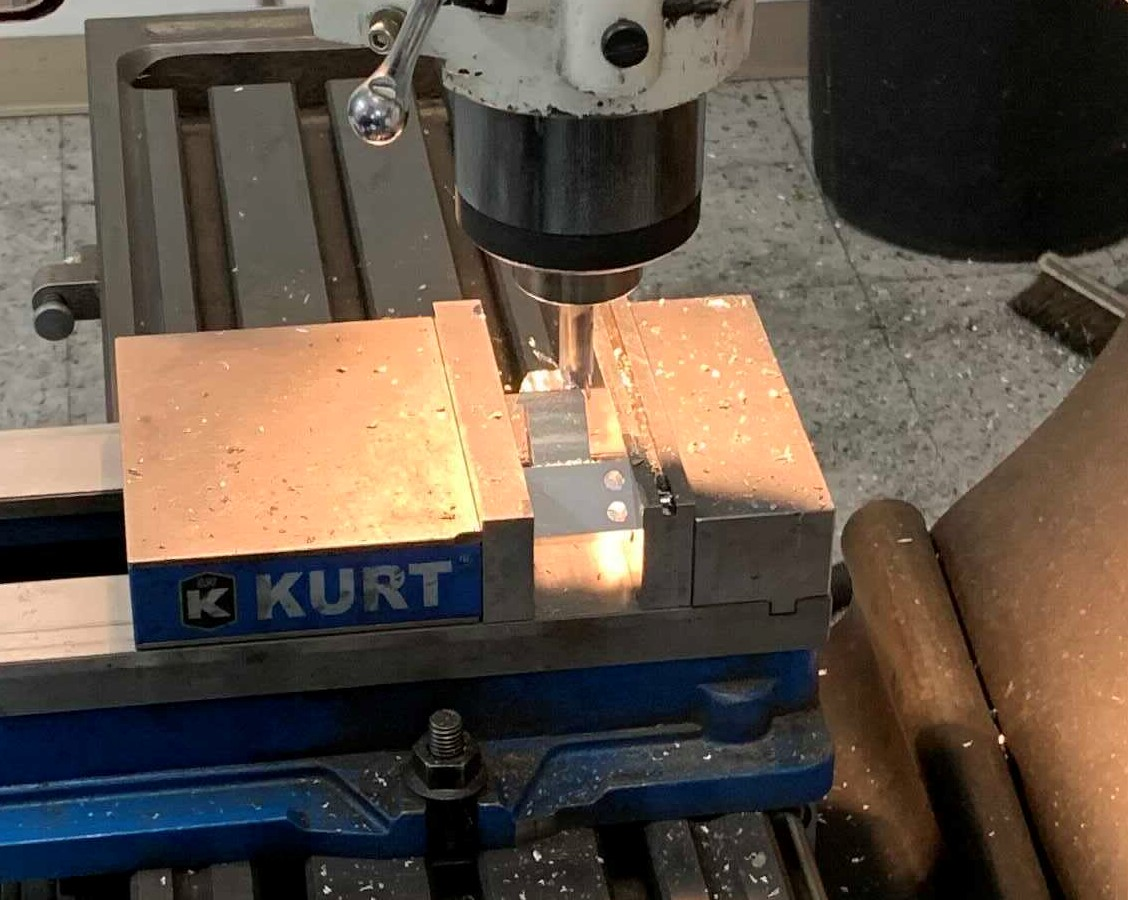
\includegraphics[width=\textwidth]{27_03-04/images/latchcut.jpg}
  \caption{Cutting the latch piece}
  \label{fig:Latchcut}
  \end{subfigure}
  \caption{New Latch}
  \end{figure}

\subsection{Cutting a New Latch Piece}
%! things
During the team reflection after NorCals, one obvious recurring problem pointed out was the inconsistent initial latch height. The problem was that the robot was barely four inches off the ground at the start of the game. The original solution to this was to make skids that pressed the robot away from the lander, however these proved to only help a little because of the flex of the poly-carbonate on the lander. The skids couldn't be moved out farther since the robot was already near the 18.To fix this Ashlin created CAD of a latch that was an inch lower that would give the robot enough hanging height, without impacting the lifts over all throw as shown in figure \ref{fig:Latch}. The team discussed this with Dan and he agreed that this was the best solution, Ashlin then went to cut the piece out at GSS with Dan a few days later, as shown in figure  \ref{fig:Latchcut}. Once the piece was cut, Aidan and Oren put it on the new lift and tested it out. It proved to be very effective and raised the starting height to almost 5 inches and didn't impact the lift's movement or throw.


  
\begin{figure}[h!]
\centering
\begin{subfigure}{.34\textwidth}
  \centering
  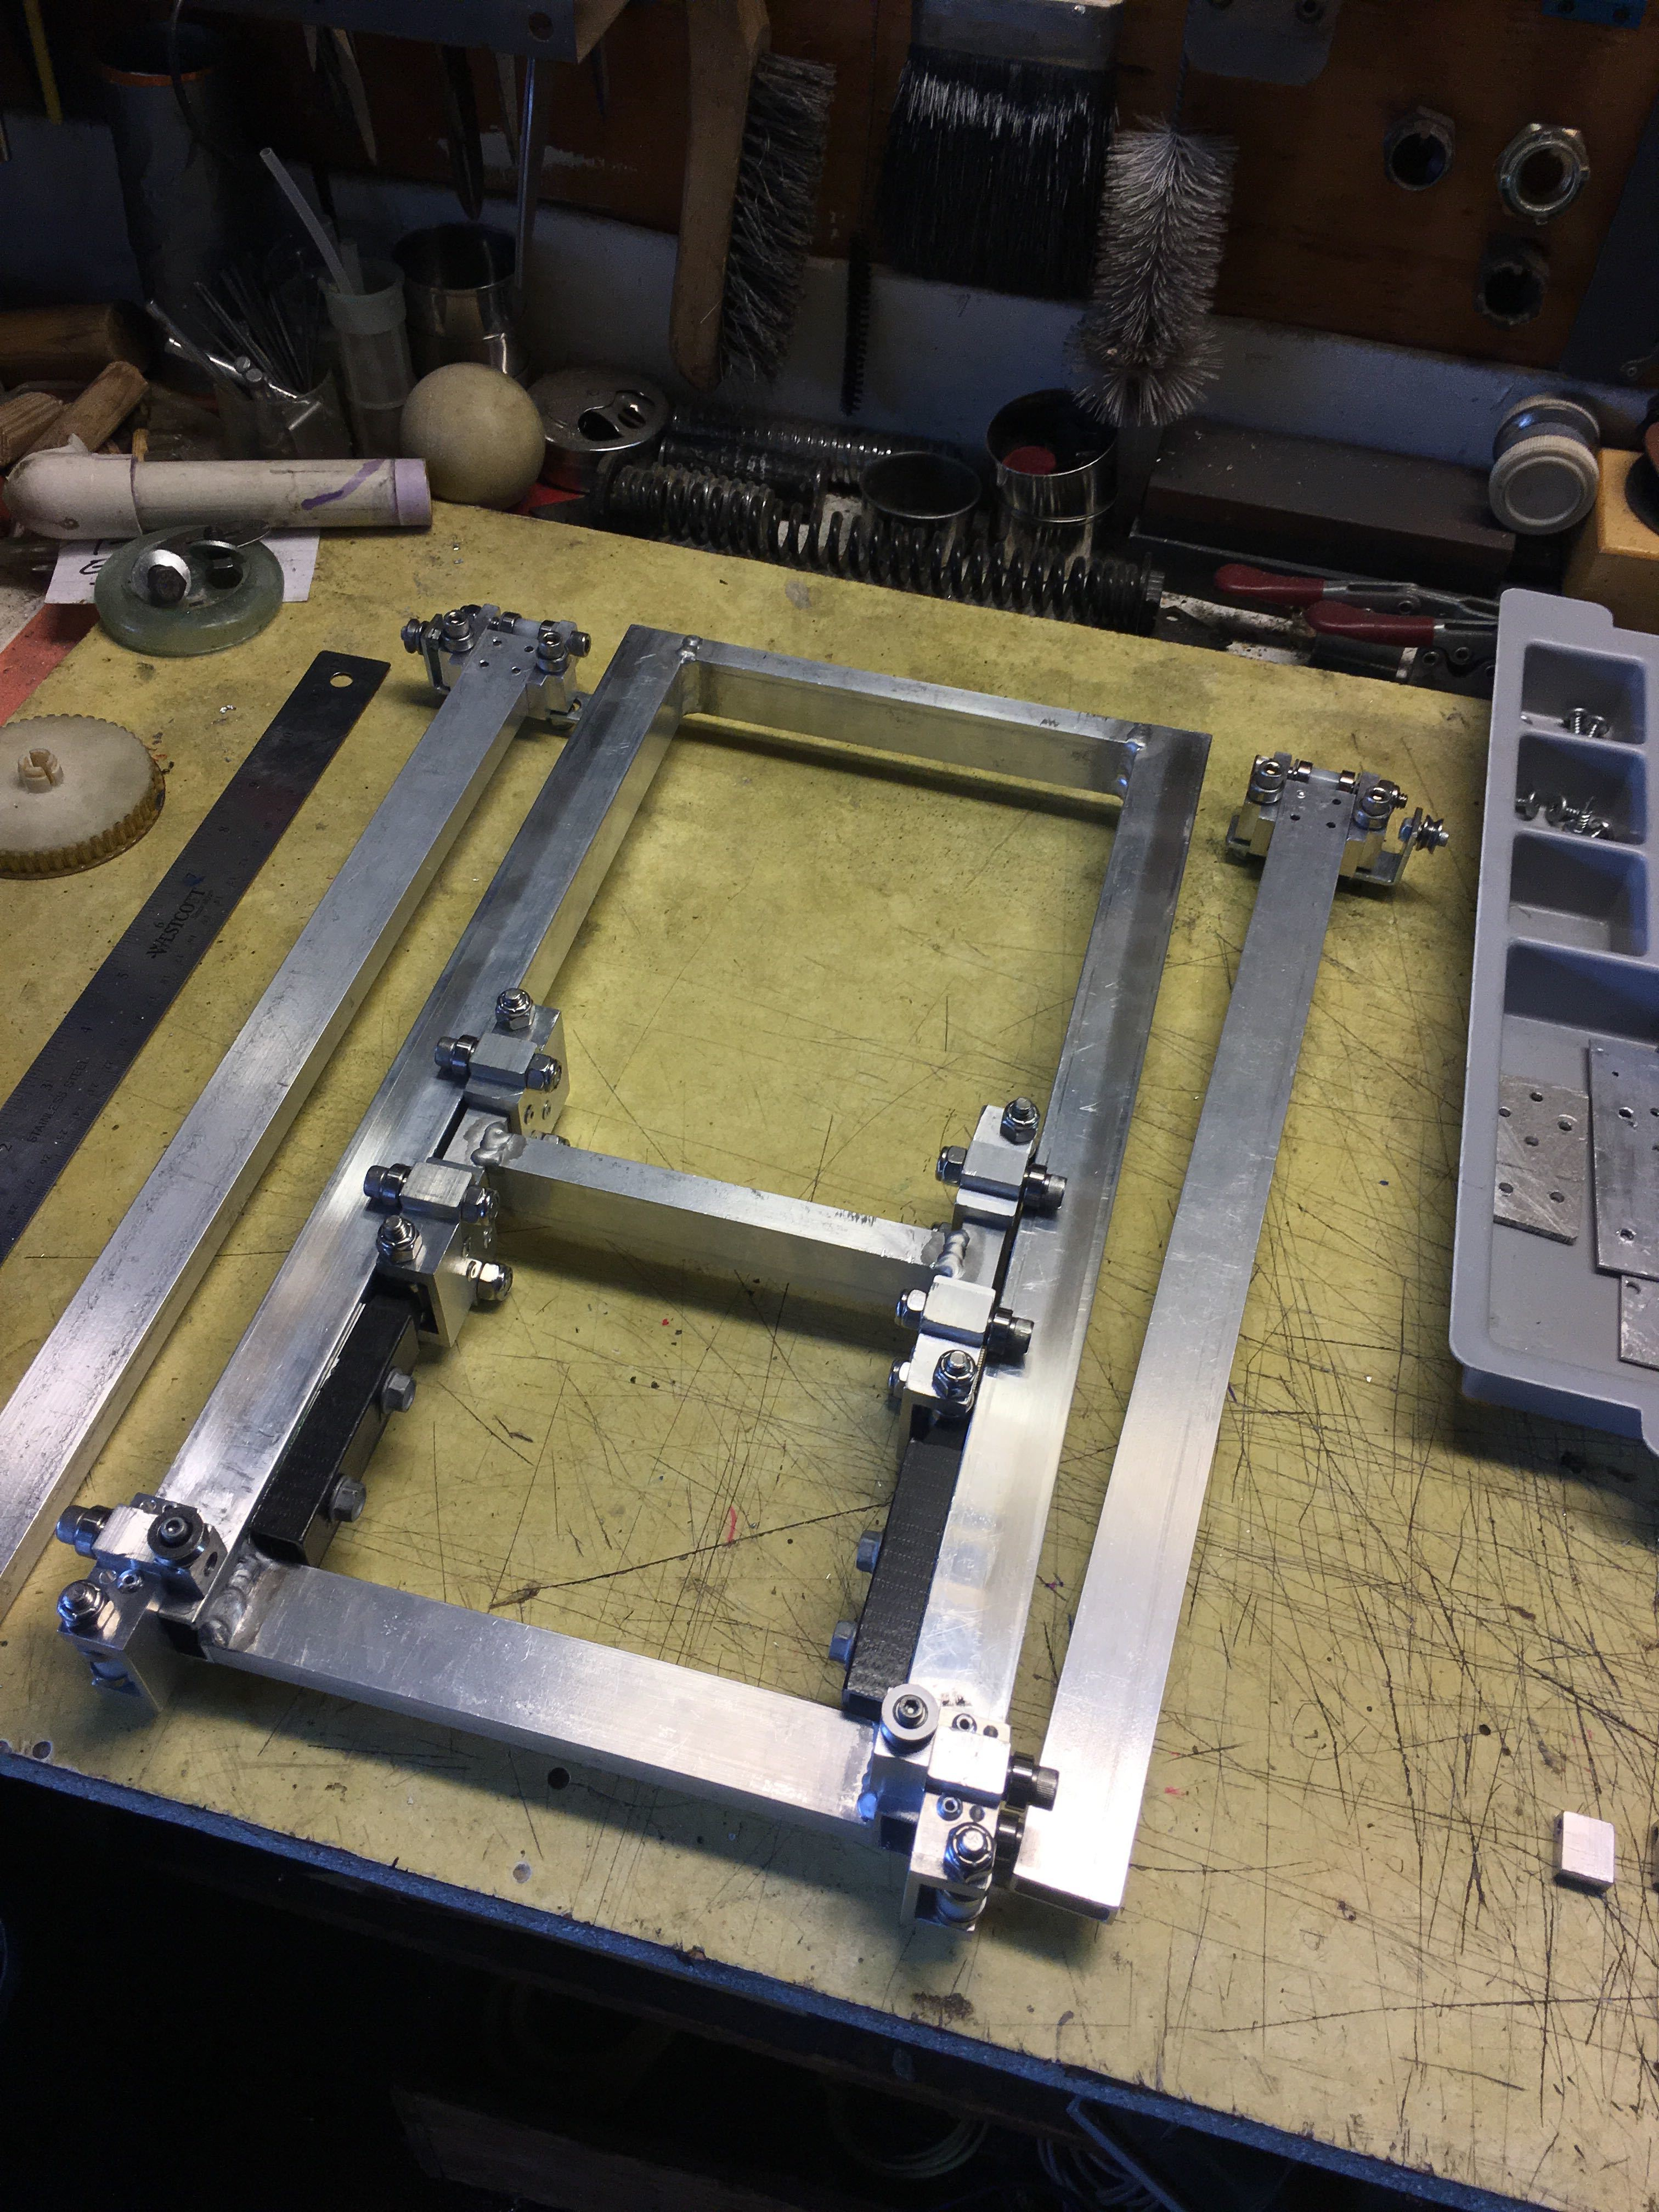
\includegraphics[width=\textwidth]{27_03-04/images/Lift2.JPG}
  \caption{Lift Assembly V.2}
  \label{fig:lift2}
 \end{subfigure}
\begin{subfigure}{.45\textwidth}
  \centering
  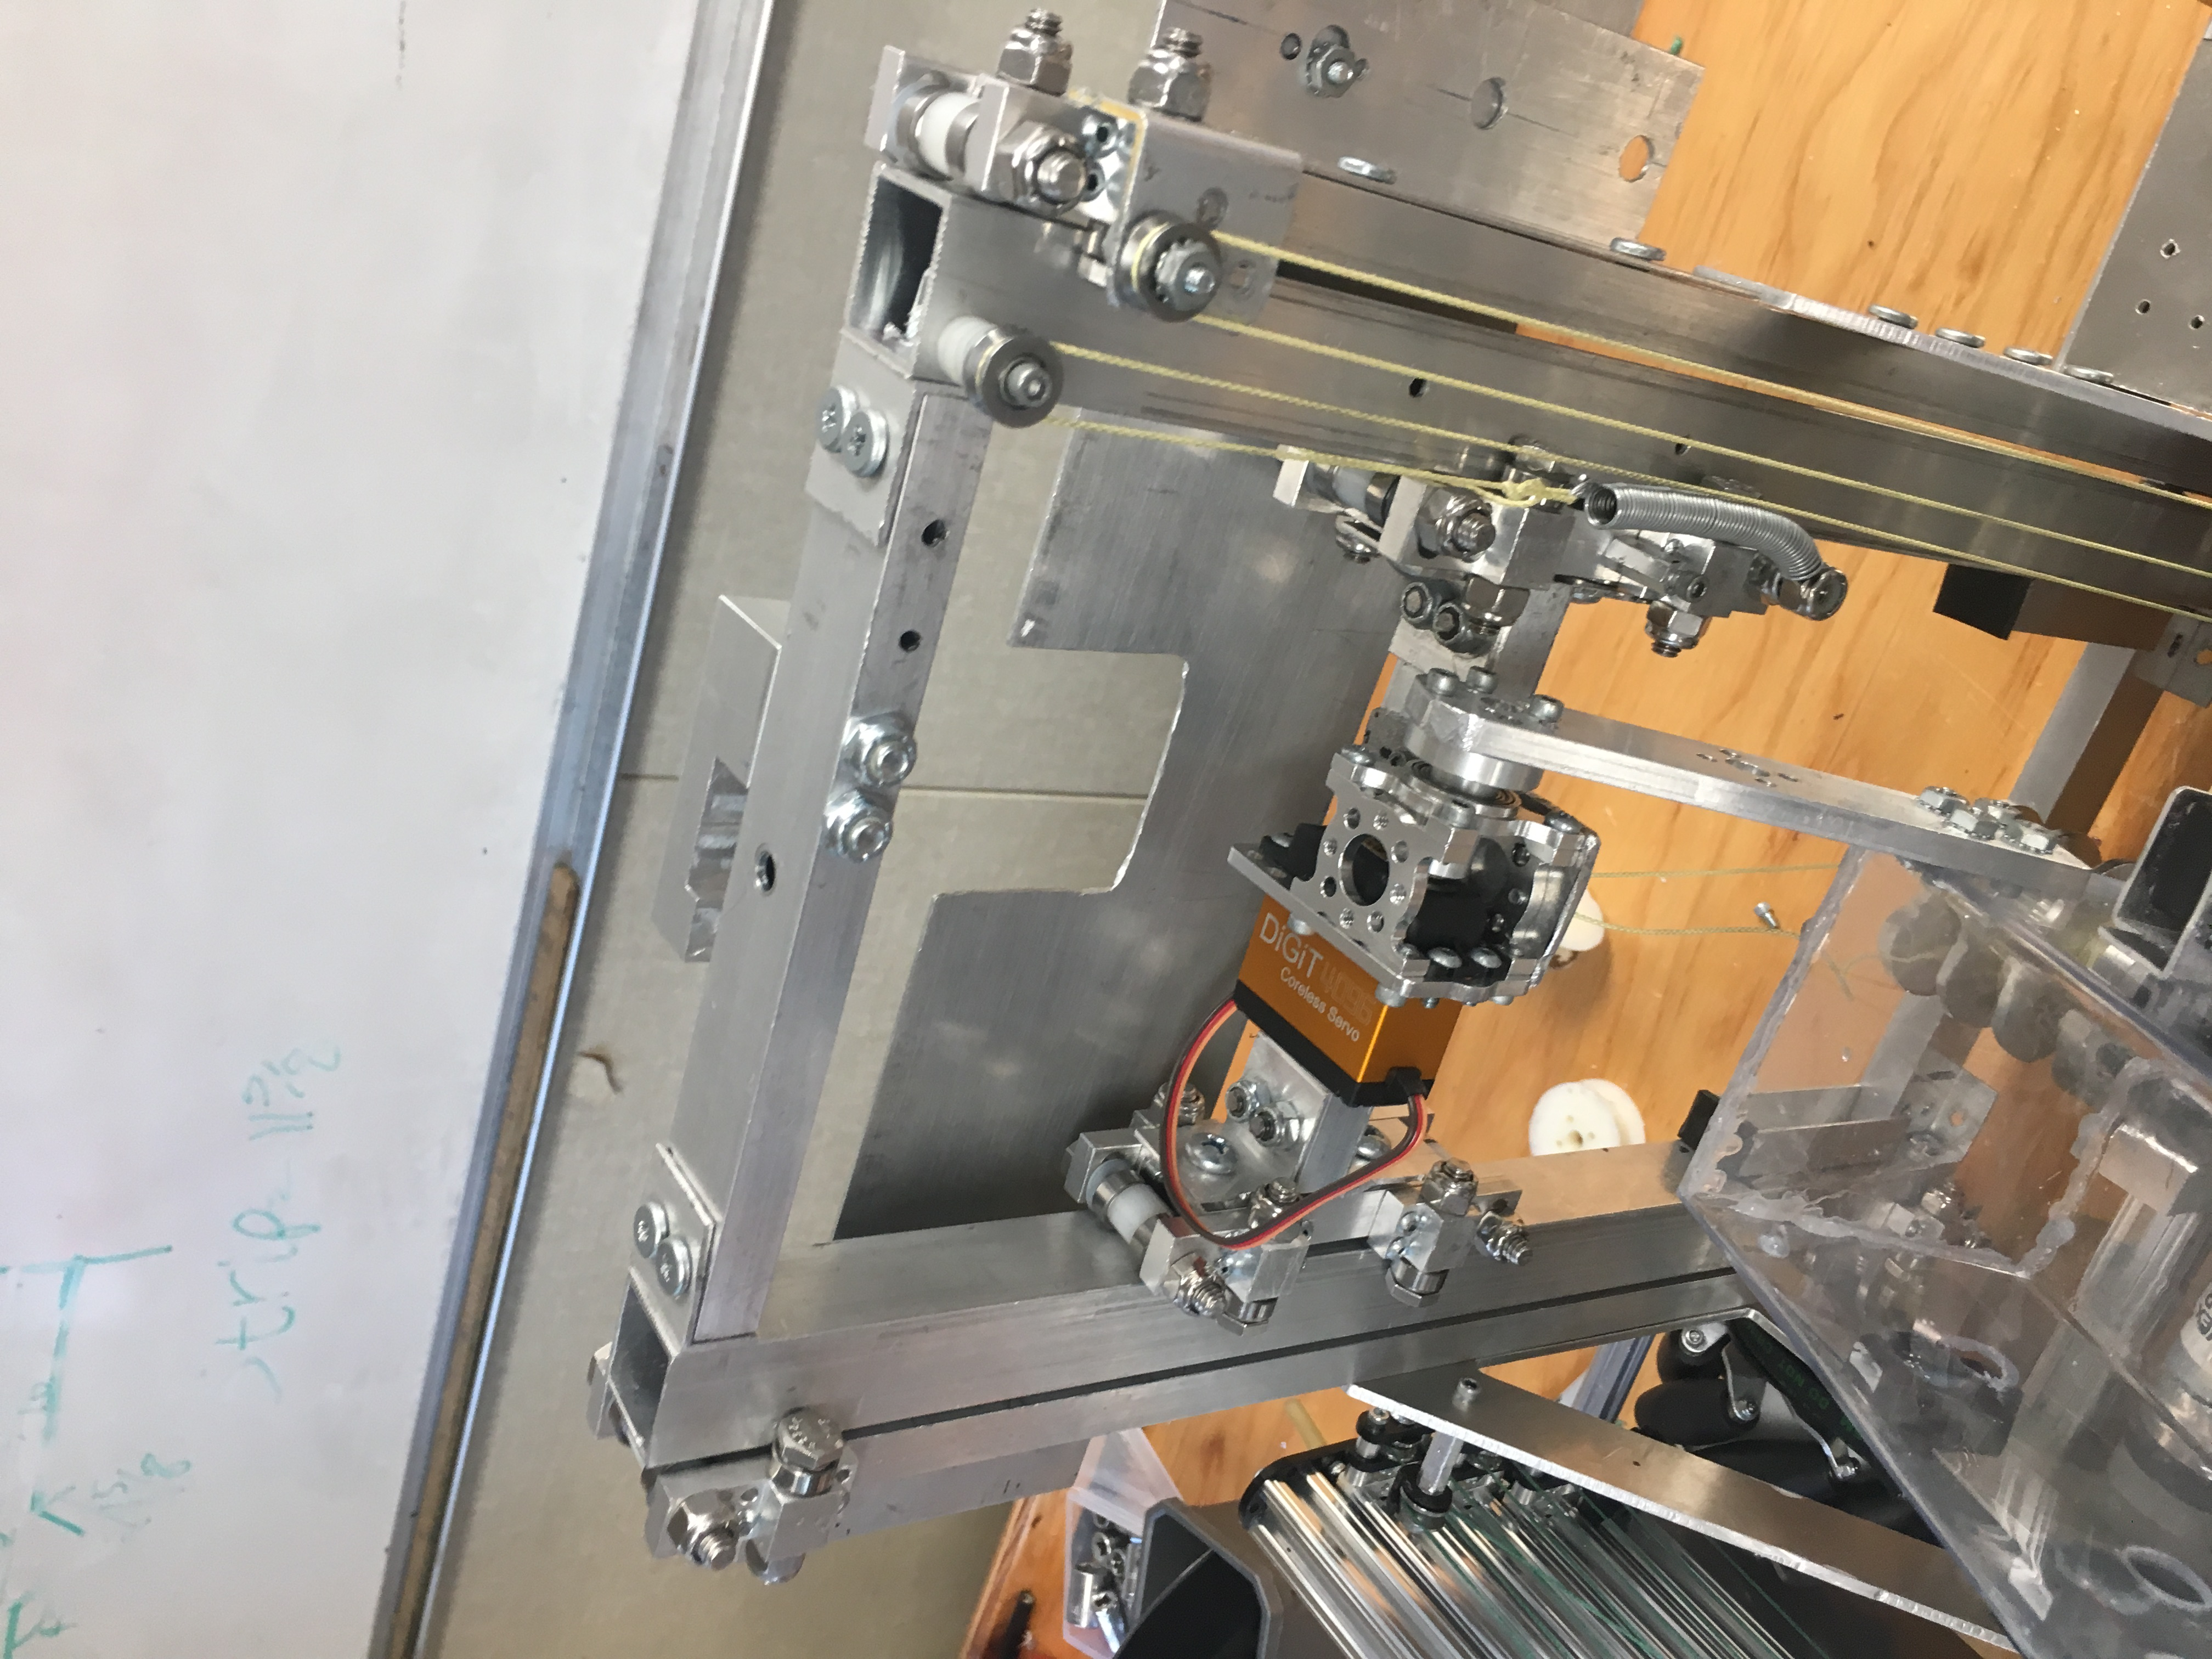
\includegraphics[width=\textwidth,angle=-90]{27_03-04/images/Lift1.JPG}
  \caption{Lift Assembly V.1}
  \label{fig:lift1}
  \end{subfigure}
  \begin{subfigure}{.45\textwidth}
    \centering
    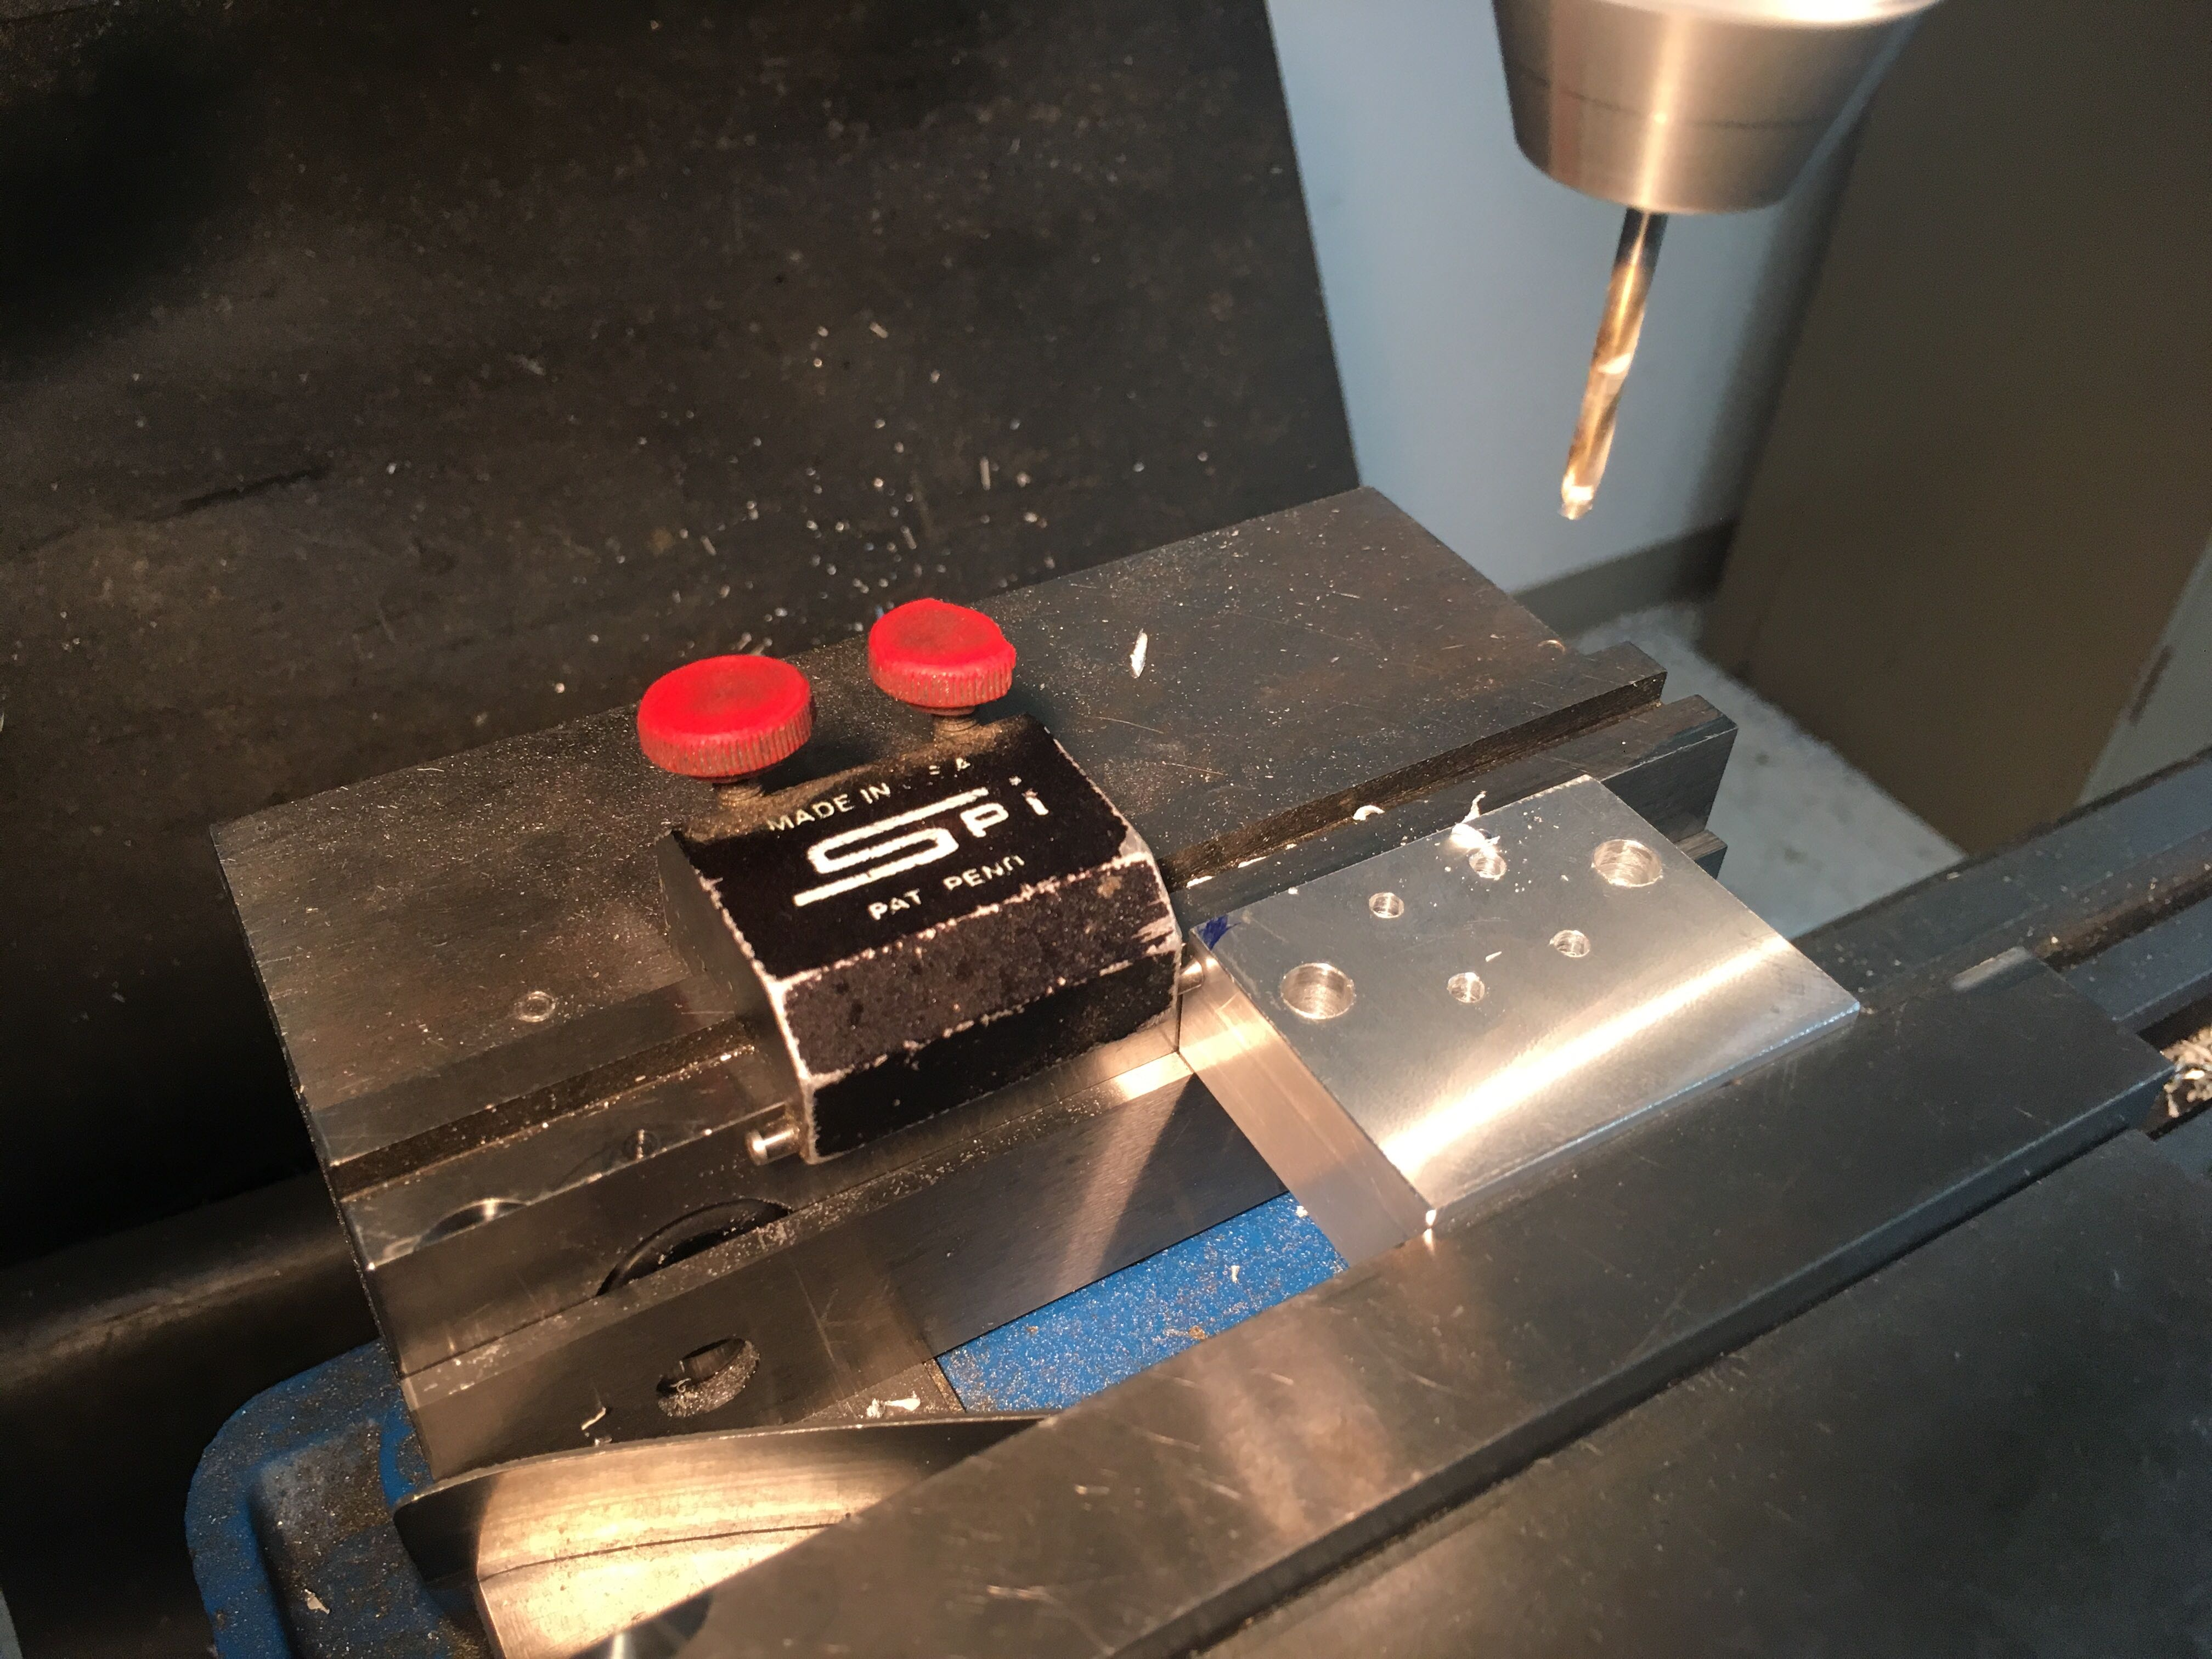
\includegraphics[width=\textwidth]{27_03-04/images/Drill.JPG}
    \caption{Drilling Out Bearing Holes}
    \label{fig:DrillHoles}
  \end{subfigure}
  \caption{Lift Assemblies}
  \end{figure}

\subsection{Lift Assembly 2.0}
%! thing
Since ACME qualified for Worlds, Oren went about assembling lift 2.0. After the NorCal tournament it became very evident that the new lift was very necessary, along with the addition of two new sensors to help during auto and teleop. These sensors were add with the intention to help zero the bottom position of the lift, along with helping find the set point for latching the robot. One sensor was mounted to the center carriage, the other to the bottom of the outside frame. The assembling process as a whole, was very straight forward due to fewer parts to the assembly and tighter manufacturing tolerances on all the moving components \ref{fig:lift2} \ref{fig:lift1}. When assembling it, the Oren noticed that there was a lot of friction between the bearings and the runners, this friction was caused by the machined part's tolerances that were based off CAD. Which in actuality was proven to be to tight, this was fixed by drilling out the bolt holes on all the bearing blocks 50 thousandths \ref{fig:DrillHoles} to ensure a smooth operation. Once completed the lift was ready to be easily bolted on to the robot and wired to run.         

\begin{figure}
    \centering
    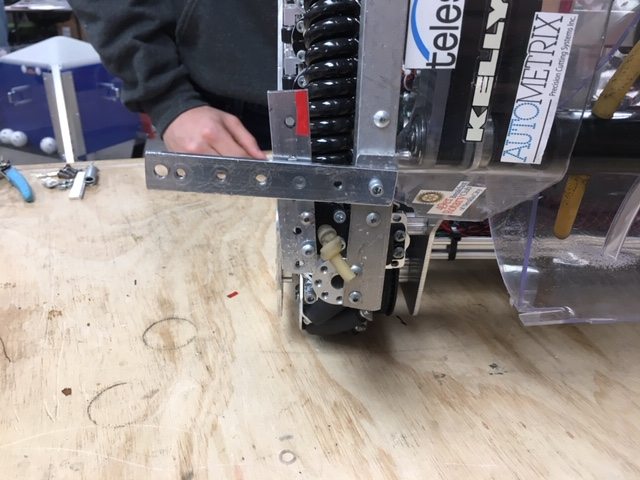
\includegraphics[width= 0.5 \textwidth]{27_03-04/images/rakemarker.JPG}
    \caption{Proof of concept for marker deployment from rake}
    \label{fig:Rake marker proof of concept}
\end{figure}

\subsection{New Team Marker Placement}
%! thing
Even with the flawless auto performance at NorCals, the team still saw places of improvement. The team mainly wanted to cut down on the time it took to complete all the tasks in auto. The main reason being that ACME wanted to start cycling in auto. The team wanted to start cycling in auto because the further the team advanced in the season, the more every point count would count. To do this however, ACME would have to reduce the time it took to complete all tasks in auto if they wanted to begin auto cycling. One of the ways ACME thought they could save the most was a faster marker deployment method. If they could deploy their team marker without having to go to the depot and then to the crater; they could save a lot of time. The team thought that the best way to do this might be to have the rake deploy the marker; since it was the farthest extending horizontal appendage. This presented a challenge, however, because their was not much space to add mechanisms to accomplish this. Jon and Shawn took on this challenge and quickly began coming up with ideas to solve the issue. At first they tried using the existing hook on the team marker to simply attach it to the top of the rake in the stowed position. The idea being when the rake deployed, the marker would simply slide off. This proved to be unreliable and caused the marker to fall very close to the depot's edge, so it was scrapped. Shawn and Jon went through several other ideas until they finally settled on a design. The design they settled on was a bracket mounted on the X-rail that didn't allow the marker to fall off with an L bracket mounted to the rake that slid underneath the marker. When the rake began to rotate, the marker be pushed up and off the rake arm. After a proof of concept, Jon and Shawn decided it was reliable and set to building the final version.

\end{document}
